\documentclass[fr]{../../../../../../eplexam}

\usepackage{stanli}

\hypertitle{MSD}{6}{MECA}{1100}{2018}{Juin}{Majeure}
{Martin Braquet}
{Issam Doghri}

\section{Théorie}
\begin{enumerate}
 \item On considère la structure représentée sur la figure 1 de l'exercice 2. On souhaite calculer le déplacement horizontal au mileu de la poutre, par deux théorèmes: (1) Maxwell-Betti, et (2) Castigliano. Pour chacun de ces théorèmes, expliquer et illustrer graphiquement la méthode de résolution, mais \textbf{sans} effectuer les calculs.
 
 \item Un système à un DDL (masse et ressort) est soumis à une force axiale $F\:\cos(\omega t)$. On ne demande \textbf{pas} d'effectuer tous les calculs, mais uniquement ceux qui permettent de: (1) montrer la différence avec le cas de vibration libre, et (2) illustrer le phénomène de résonance. 
\end{enumerate}

\section{}
On se propose d'étudier une poutre de longueur $L$ encastrée en A, simplement appuyée en B (déplacement horizontal en B nul) et soumise à une force de compression verticale $F$ appliquée à une distance $D$ du point B (voir figure \ref{q1}).

\begin{figure}[!h]
 \centering
 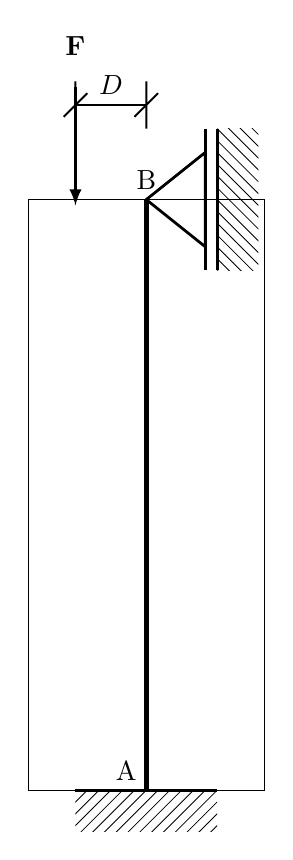
\begin{tikzpicture}[scale=1.5]
    \scaling {1.5};
    \centering
    \draw (-1,0) rectangle (1,5);
    \point{a}{0}{0}
    \point{b}{0}{5}
    \point{c}{-0.6}{4.8}
    \beam {4}{a}{b};
    \support {3}{a};
    \support {2}{b}[90];
    \load {1}{c}[90];
    \dimensioning {1}{b}{c}{5.8}[$D$];
    \notation {1}{c}{$\vv{\mathbf{F}}$}[above=2];
    \notation {1}{a}{A}[above left];
    \notation {1}{b}{B}[above];
 \end{tikzpicture}
 \caption{}
 \label{q1}
\end{figure}

\subsection*{Partie I}
Dans cette partie on étudie la structure par la théorie des poutres classique sans se soucier d'une éventuelle instabilité.
\begin{enumerate}
 \item Calculer les réactions aux appuis A et B en choisissant la réaction au point B comme inconnue hyperstatique (on utilise Castigliano et on ne regarde que l'énergie de déformation due au moment fléchissant).
 \item Dessiner les diagrammes des efforts internes en indiquant les signes et les valeurs remarquables.
\end{enumerate}

\subsection{Partie II}
Dans cette partie on se propose d'étudier la stabilité de la structure.
\begin{enumerate}
 \item Ecrire les équations régissant le problème de stabilité.
 \item Intégrer l'équation différentielle et calculer les constantes d'intégration.
 \item Donner l'expression de la flèche en milieu de poutre et montrer qu'elle tend vers l'infini si $F$ atteint une valeur critique que l'on calculera (une solution approchée de $\tan x=x$ est $x=4.493$).
\end{enumerate}

\section{}
\textit{Toutes les questions, à l'exception de la question 2, peuvent être traitées indépendamment.}\\

On étudie les vibrations libres d'une structure comprenant deux poutres rigides de masse distribuée $m$ et de longueur $2L$. Les \textbf{deux} poutres sont portées par deux \textbf{rotules fixes} et elles sont reliées entre elles par des ressorts linéaires de raideurs $k$ et $3k/4$. Les poutres forment des angles $\varphi$ et $\theta$ par rapport à la verticale. Les ressorts sont sans sontrainte lorsque les deux éléments sont verticaux ($\varphi=\theta=0$).

On choissit comme coordonnées généralisées:
\[
 \underset{\sim}{x}=\begin{pmatrix}
L\,\varphi \\ L\,\theta
\end{pmatrix}
\]
qui représentent les positions des poutres par rapport aux positions d'équilibre statique. On suppose les ressorts verticaux.

\begin{figure}[!h]
 \centering
 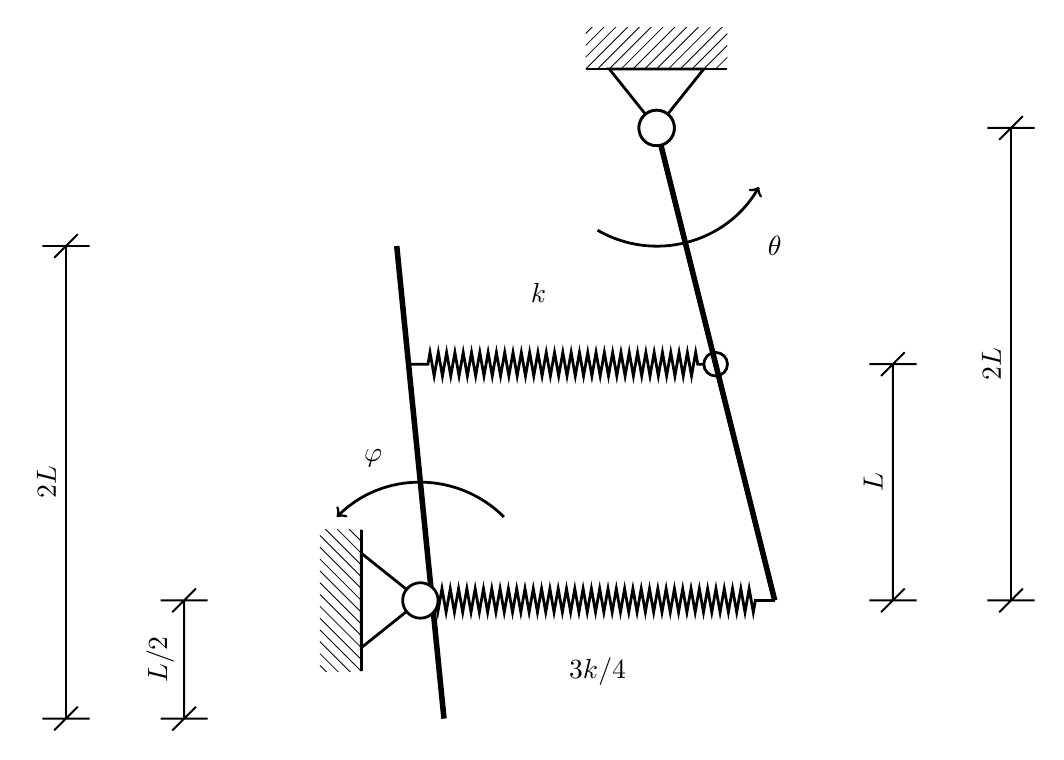
\begin{tikzpicture}[scale=1.5]
  \scaling {1.5};
  \point {a}{0}{0};
  \point {b}{0.2}{-1};
  \point {c}{-0.2}{3};
  \point {d}{-0.1}{2};
  \point {e}{2}{4};
  \point {f}{3}{0};
  \dsupport {4}{d}[-2.6][0][0];
  \dsupport {4}{f}[3][0][0];
  \support {1}{a}[-90];
  \beam {4}{b}{c};
  \load {3}{a}[45][90][1];
  \hinge {1}{a};
  \support {1}{e}[180];
  \hinge {1}{e};
  \beam {4}{e}{f};
  \load {2}{e}[-30][-90][1];
  \node at (1,2.6){$k$};
  \node at (-0.4,1.2){$\varphi$};
  \node at (3,3){$\theta$};
  \node at (1.5,-0.6){$3k/4$};
  \dimensioning {2}{b}{a}{-2}[$L/2$];
  \dimensioning {2}{b}{c}{-3}[$2L$];
  \dimensioning {2}{f}{d}{4}[$L$];
  \dimensioning {2}{f}{e}{5}[$2L$];
  \hinge {1}{e};
 \end{tikzpicture}
 \caption{}
 \label{q1}
\end{figure}

\begin{enumerate}
 \item Calculez les modes propres du système en utilisant les matrices de masse et de raideur suivantes:
 \[
  \mathbf{M}=m\begin{pmatrix} 7/12 & 0 \\ 0 & 4/3 \end{pmatrix}
  \qquad
  \mathbf{K}=k\begin{pmatrix} 3/5 & 1 \\ 1 & 24/5 \end{pmatrix}
 \]
 \item A partir de votre réponse à la question précédente, donnez l'expression mathématique de l'évolution temporelle des coordonnées généralisées $\underset{\sim}{x}(t)$ lorsque les deux poutres sont parallèles en position initiale et ont une vitesse initiale nulle.
 \item Calculez le coefficient de Rayleigh pour le vecteur propre $\begin{pmatrix} 1 \\ -1 \end{pmatrix}$. Que représente-t-il?
 \item Vérifiez que les matrices de masse et de raideur correspondant à de petites oscillations autour de la position d'équilibre verticale et lorsque $5\,mg=4\,kl$, ont les expressions données dans la question 1. On rappelle les équations de Lagrange:
 \[
  L=\mathrm{énergie \: cinétique - énergie \: potentielle}
  \]
  \[
  \frac{d}{dt}\frac{\partial L}{\partial \dot{x}_i}-\frac{\partial L}{\partial x_i}=0
 \]
 avec $x_i$ les composantes des coordonnées généralisées.
\end{enumerate}





\end{document}
